\documentclass[../../main/main.tex]{subfiles}
\graphicspath{{./figures/}}

\dominitoc
\faketableofcontents

\renewcommand{\mtcSfont}{\small\bfseries}
\renewcommand{\mtcSSfont}{\footnotesize}
\mtcsettitle{minitoc}{}
\mtcsetrules{*}{off}

\makeatletter
\renewcommand{\@chapapp}{Thermodynamique -- chapitre}
\makeatother

% \toggletrue{student}
% \toggletrue{corrige}
% \renewcommand{\mycol}{black}
% \renewcommand{\mycol}{gray}

\hfuzz=5.003pt

\begin{document}
\setcounter{chapter}{2}

\settype{book}
\settype{prof}
\settype{stud}

\chapter{Premier principe de la thermodynamique}

\epigraph{\openquote\textit{%
		A theory is the more impressive the greater the simplicity of its premises,
		the more different kinds of things it relates, and the more extended its
		area of applicability. Therefore the deep impression that classical
		thermodynamics made upon me. It is the only physical theory of universal
		content which I am convinced will never be overthrown, within the framework
		of applicability of its basic concepts.
	}\closequote}{Albert \textsc{Einstein}, \textit{Autobiographical notes}, 1949}

\vspace*{\fill}

\begin{tcn}*(appl)<ctc>{\iconsomm~Sommaire}
	\let\item\olditem
	\vspace{-15pt}
	\minitoc
	\vspace{-25pt}
\end{tcn}

\begin{tcn}*[sidebyside, sidebyside align=top,
		fontupper=\small, fontlower=\small](appl)<ctb>"how"'t'{Capacités exigibles}
	\begin{itemize}[label=\rcheck]
		\item Définir un système fermé et établir pour ce système un bilan
		      énergétique faisant intervenir travail et transfert thermique.

		\item Distinguer le statut de la variation de l'énergie interne du statut des
		      termes d'échange.

		\item Calculer le transfert thermique sur un chemin donné connaissant le
		      travail et la variation de l'énergie interne.

		\item Utiliser le premier principe de la thermodynamique entre deux états
		      voisins.

		\item Exploiter l'extensivité de l'énergie interne.

		\item Citer l'ordre de grandeur de la capacité thermique massique de l'eau
		      liquide.
	\end{itemize}
	\tcblower
	\begin{itemize}[label=\rcheck]

		\item Exprimer le premier principe sous forme de bilan d'enthalpie dans le cas
		      d'une transformation monobare avec équilibre mécanique dans l'état initial
		      et dans l'état final.

		\item Exprimer l'enthalpie $H_m(T)$ du gaz parfait à partir de l'énergie
		      interne.

		\item Justifier que l'enthalpie $H_m$ d'une phase condensée peu compressible
		      et peu dilatable peut être considérée comme une fonction de l'unique
		      variable T.

		\item Exploiter l'extensivité de l'enthalpie et réaliser des bilans
		      énergétiques en prenant en compte des transitions de phases.
	\end{itemize}
\end{tcn}

\vspace*{\fill}

\newpage

\vspace*{\fill}
% {
% \begin{boxes}
\begin{tcn}[sidebyside, fontupper=\small, fontlower=\small](appl)<ctb>"check"'t'{L'essentiel}
	\begin{tcn}(defi)<ctc>'t'{Définitions}
		\tcblistof[\paragraph*]{defi}{\hspace*{4.8pt}}
	\end{tcn}
	% \begin{tcn}(rapp)<ctc>'t'{Rappels}
	% 	\tcblistof[\paragraph*]{rapp}{\hspace*{4.8pt}}
	% \end{tcn}
	\begin{tcn}(prop)<ctc>'t'{Propriétés}
		\tcblistof[\paragraph*]{prop}{\hspace*{4.8pt}}
		\tcblistof[\paragraph*]{loi}{\hspace*{4.8pt}}
		% \tcblistof[\paragraph*]{theo}{\hspace*{4.8pt}}
	\end{tcn}
	% \begin{tcn}(coro)<ctc>'t'{Corollaires}
	%   \tcblistof[\paragraph*]{coro}{\hspace*{4.8pt}}
	% \end{tcn}
	\begin{tcn}(demo)<ctc>'t'{Démonstrations}
		\tcblistof[\paragraph*]{demo}{\hspace*{4.8pt}}
		\tcblistof[\paragraph*]{prev}{\hspace*{4.8pt}}
	\end{tcn}
	% \begin{tcn}(inte)<ctc>'t'{Interprétations}
	%   \tcblistof[\paragraph*]{inte}{\hspace*{4.8pt}}
	% \end{tcn}
	% \begin{tcn}(tool)<ctc>'t'{Outils}
	% 	\tcblistof[\paragraph*]{tool}{\hspace*{4.8pt}}
	% \end{tcn}
	% \begin{tcn}(nota)<ctc>'t'{Notations}
	%   \tcblistof[\paragraph*]{nota}{\hspace*{4.8pt}}
	% \end{tcn}
	% \begin{tcn}(appl)<ctc>'t'{Applications}
	%   \tcblistof[\paragraph*]{appl}{\hspace*{4.8pt}}
	% \end{tcn}
	% \begin{tcn}(rema)<ctc>'t'{Remarques}
	%   \tcblistof[\paragraph*]{rema}{\hspace*{4.8pt}}
	% \end{tcn}
	% \begin{tcn}(exem)<ctc>'t'{Exemples}
	%   \tcblistof[\paragraph*]{exem}{\hspace*{4.8pt}}
	% \end{tcn}
	% \begin{tcn}*(ror)<ctc>"hart"'t'{Points importants}
	%   \tcblistof[\paragraph*]{ror}{\hspace*{4.8pt}}
	% \end{tcn}
	% \begin{tcn}(impo)<ctc>'t'{Erreurs communes}
	%   \tcblistof[\paragraph*]{impo}{\hspace*{4.8pt}}
	% \end{tcn}
	\tcblower
	% \begin{tcn}(defi)<ctc>'t'{Définitions}
	%   \tcblistof[\paragraph*]{defi}{\hspace*{4.8pt}}
	% \end{tcn}
	% \begin{tcn}(rapp)<ctc>'t'{Rappels}
	%   \tcblistof[\paragraph*]{rapp}{\hspace*{4.8pt}}
	% \end{tcn}
	% \begin{tcn}(prop)<ctc>'t'{Propriétés}
	%   \tcblistof[\paragraph*]{prop}{\hspace*{4.8pt}}
	%   \tcblistof[\paragraph*]{loi}{\hspace*{4.8pt}}
	%   \tcblistof[\paragraph*]{theo}{\hspace*{4.8pt}}
	% \end{tcn}
	% \begin{tcn}(coro)<ctc>'t'{Corollaires}
	%   \tcblistof[\paragraph*]{coro}{\hspace*{4.8pt}}
	% \end{tcn}
	% \begin{tcn}(demo)<ctc>'t'{Démonstrations}
	% 	\tcblistof[\paragraph*]{demo}{\hspace*{4.8pt}}
	% 	\tcblistof[\paragraph*]{prev}{\hspace*{4.8pt}}
	% \end{tcn}
	\begin{tcn}(inte)<ctc>'t'{Interprétations}
		\tcblistof[\paragraph*]{inte}{\hspace*{4.8pt}}
	\end{tcn}
	\begin{tcn}(inte)<ctc>'t'{Implications}
		\tcblistof[\paragraph*]{impl}{\hspace*{4.8pt}}
	\end{tcn}
	% \begin{tcn}(tool)<ctc>'t'{Outils}
	%   \tcblistof[\paragraph*]{tool}{\hspace*{4.8pt}}
	% \end{tcn}
	% \begin{tcn}(nota)<ctc>'t'{Notations}
	%   \tcblistof[\paragraph*]{nota}{\hspace*{4.8pt}}
	% \end{tcn}
	\begin{tcn}(appl)<ctc>'t'{Applications}
		\tcblistof[\paragraph*]{appl}{\hspace*{4.8pt}}
	\end{tcn}
	% \begin{tcn}(rema)<ctc>'t'{Remarques}
	%   \tcblistof[\paragraph*]{rema}{\hspace*{4.8pt}}
	% \end{tcn}
	% \begin{tcn}(exem)<ctc>'t'{Exemples}
	% 	\tcblistof[\paragraph*]{exem}{\hspace*{4.8pt}}
	% \end{tcn}
	\begin{tcn}*(ror)<ctc>"hart"'t'{Points importants}
		\tcblistof[\paragraph*]{ror}{\hspace*{4.8pt}}
	\end{tcn}
	\begin{tcn}(impo)<ctc>'t'{Erreurs communes}
		\tcblistof[\paragraph*]{impo}{\hspace*{4.8pt}}
	\end{tcn}
\end{tcn}
% \end{boxes}
% }%

\vspace*{\fill}
\newpage

\section{Énoncé du premier principe}
\subsection{Énoncé général}
\begin{tcb}[sidebyside, righthand ratio=.2](rapp){Énergie totale d'un système}
	L'énergie d'un système thermodynamique a deux composantes~:
	\begin{itemize}
		\item[b]{Macroscopique}~: c'est l'énergie mécanique $\Ec_m = \Ec_c + \Ec_p$~;
		\item[b]{Microscopique}~: c'est l'énergie interne $U = e_c + e_p$.
	\end{itemize}
	Ce sont des \textbf{grandeurs d'état extensives et additives}.
	\tcblower
	\[
		\boxed{\Ec = \Ec_m + U}
	\]
\end{tcb}

La variation d'énergie d'un système peut alors se mettre sous la forme
\[
	\Delta{\Ec} = \Ec\ind{échangée}
\]
c'est-à-dire que tout variation d'énergie ne provient que d'un échange avec
l'extérieur. On rappelle que dans ce cas, $E\ind{échangée}$ est l'énergie
\textbf{reçue} par le système étudié. Nous obtenons alors le premier principe de
la thermodynamique~:

\begin{tcb*}[%
		list entry={\hspace*{-20pt}\protect\rcheck~~Premier principe de la thermo.}%
	](prop){Premier principe de la thermodynamique}
	Un système thermodynamique \textbf{fermé} ne peut céder ou recevoir de
	l'énergie que de deux manières~:
	\begin{itemize}
		\item \textit{via} des interactions \textbf{macroscopique} sous forme de
		      \xul{\psw{\textbf{travail}}}, noté \psw{$W$}~;
		\item \textit{via} des interactions \textbf{microscopiques} sous forme de
		      \xul{\psw{\textbf{transfert thermique}}}, noté \psw{$Q$}.
	\end{itemize}
	\xul{\psw{$W$}} et \xul{\psw{$Q$}} ne sont \textbf{pas} des grandeurs d'état
	mais \textbf{dépendent du chemin suivi}. Ainsi, la conservation de l'énergie
	impose~:
	\smallbreak
	\begin{isd}[interior hidden](prop)
		\tcbsubtitle{\fatbox{\textbf{Général}}}
		\psw{%
			\[
				\boxed{\Delta{\Ec} = W + Q}
			\]
		}%
		\vspace{-15pt}
		\tcblower
		\tcbsubtitle{\fatbox{\textbf{Repos macroscopique}}}
		\psw{%
			\[
				\boxed{\Delta{U} = W + Q}
			\]
		}%
		\vspace{-15pt}
	\end{isd}
\end{tcb*}

On se placera la plupart du temps dans un état de repos macroscopique~:
$\Delta{\Ec_c} = \Delta{\Ec_p} = 0$.

\subsection{Première loi de \textsc{Joule}}

\begin{tcb*}[sidebyside, sidebyside align=top](loi){Première loi de \textsc{Joule}}
	\tcbsubtitle{\fatbox{\textbf{Énoncé}}}
	Les gaz parfaits et les phases condensées vérifient la première loi de
	\textsc{Joule}~: leur \textbf{variation d'énergie interne molaire} ou massique
	ne dépend \textbf{que de la température}~:
	\psw{%
		\[
			U_m = U_m(T)
		\]
	}%
	\vspace{-15pt}
	\tcblower
	\tcbsubtitle{\fatbox{\textbf{Conséquence}}}
	\vspace{-15pt}
	\psw{%
		\begin{gather*}
			\dd{U} = C_V \dd{T}
			\Lra
			\Delta{U} = \int_{T_i}^{T_f} C_V \dd{T}
			\\\beforetext{$C_{V,m} = \cte \Ra$}
			\boxed{\Delta{U} = C_V\Delta{T}}
		\end{gather*}
	}%
	\vspace{-15pt}
\end{tcb*}

\begin{tcb}(rapp)<lftt>{$U_m\sup{G.P.}$ et $U_m\sup{cond}$}
	On avait déjà établit pour le \textbf{gaz parfait} et les \textbf{phases
		condensées}~:
	\psw{%
		\[
			U_m\sup{G.P.} = \frac{D}{2}nRT
			\qqet
			U_m\sup{cond} = U_m(T)
		\]
	}%
	\vspace{-15pt}
\end{tcb}

\begin{tcb}(appl)<lftt>{Cycle de \textsc{Lenoir}}
	On reprend le cycle établi dans le chapitre précédent, constitué d'une
	isochore AB, d'une isotherme BC puis d'une isobare CA.
	\begin{enumerate}[start=4, label=\sqenumi]
		\item Calculer les transferts thermiques associés aux transformations AB, BC
		      et CA, puis sur le cycle. Commenter le résultat.
	\end{enumerate}
	\tcblower
	\begin{enumerate}[start=4, label=\sqenumi]
		\item
		      \begin{isd}[sidebyside align=top]
			      \begin{itemize}
				      \item On calcule les $\Delta{U}$~:
				            \begin{align*}
					            \Delta{U}\ind{AB} & =
					            \psw{C_V\Delta{T} = \frac{5}{2}nR(T\ind{B} - T\ind{A}) = \SI{7.0}{kJ}}
					            \\
					            \Delta{U}\ind{BC} & =
					            \psw{\frac{5}{2}nR(T\ind{C} - T\ind{B}) = 0}
					            \\
					            \Delta{U}\ind{CA} & =
					            \psw{\frac{5}{2}nR(T\ind{A} - T\ind{C}) = \SI{-7.0}{kJ}}
				            \end{align*}
			      \end{itemize}
			      \tcblower
			      \begin{itemize}
				      \item D'où les transferts thermiques~:
				            \begin{align*}
					            Q\ind{AB} & = \psw{\Delta{U}\ind{AB} - W\ind{AB} = \SI{7.0}{kJ}}
					            \vphantom{\frac{5}{2}}
					            \\
					            Q\ind{BC} & = \psw{\Delta{U}\ind{BC} - W\ind{BC} = \SI{3.88}{kJ}}
					            \vphantom{\frac{5}{2}}
					            \\
					            Q\ind{CA} & = \psw{\Delta{U}\ind{CA} - W\ind{CA} = \SI{-9.8}{kJ}}
					            \vphantom{\frac{5}{2}}
				            \end{align*}
			      \end{itemize}
		      \end{isd}
		      \begin{gather*}
			      \beforetext{Ainsi,}
			      \setlength{\fboxsep}{3mm}
			      \boxed{\psw{Q\ind{cycle} = \SI{+1.08}{kJ}}}
		      \end{gather*}
		      Le fluide reçoit un transfert thermique \xul{\psw{\textbf{positif}}}, et
		      un travail \xul{\psw{\textbf{négatif}}}~; autrement dit il convertit un
		      transfert thermique en travail mécanique~: c'est un
		      \xul{\psw{\textbf{moteur}}}.
	\end{enumerate}
\end{tcb}

\begin{tcb*}(ror){Calcul de transferts thermiques}
	Pour un gaz parfait ou une phase condensée incompressible et indilatable, on
	connaît les expressions de $\Delta{U}$ et $\Delta{W_p}$~: on détermine donc
	$Q$ par premier principe~: $\setlength{\fboxsep}{3mm}\boxed{\psw{Q =
				\Delta{U}-Q}}$.
	\vspace{-15pt}
	\begin{center}
		\captionof{table}{Expressions de $U$, $W_p$ et $Q$ pour un gaz parfait}
		\begin{tabularx}{\linewidth}{cYYY}
			\toprule
			\textbf{Transformation}
			 &
			\textbf{Énergie interne}
			 &
			\textbf{Travail pression}
			 &
			\textbf{Transfert thermique}
			\\
			\midrule
			Isotherme
			 &
			\psw{$\Delta{U} = 0$}
			 &
			\psw{$\DS W = -nRT_0 \ln \frac{V_f}{V_i}$}
			 &
			\psw{$\DS Q = nRT_0 \ln \frac{V_f}{V_i}$}
			\\\addlinespace[0.5em]
			Isochore
			 &
			\psw{$\Delta{U} = C_V (T_f - T_i)$}
			 &
			\psw{$W = 0$}
			 &
			\psw{$Q = C_V (T_f - T_i)$}
			\\\addlinespace[1em]
			Monobare
			 &
			\psw{$\Delta{U} = C_V (T_f - T_i)$}
			 &
			\psw{$W = -P\ind{ext} (V_f - V_i)$}
			 &
			\psw{$Q = (C_V-nR)(T_f-T_i)$}
			\\
			\bottomrule
		\end{tabularx}
	\end{center}
\end{tcb*}

\subsection{Cas particuliers}
\subsubsection{Thermostat}
On peut alors justifier qu'un thermostat est un système de capacité thermique
infinie.
\begin{tcb}[sidebyside](appl)<lftt>{Thermostat}
	On jette un bloc de fer de température élevée dans un lac de température
	faible. Le système \{bloc+lac\} est isolé, et les deux phases sont
	incompressibles et indilatables. Montrer que la température du lac reste
	constante.
	\tcblower
	\psw{%
		\begin{align*}
			\Delta{U} = 0
			                                             & \Lra
			\Delta{U}\ind{lac} = -\Delta{U}\ind{bloc}
			\\\Lra
			\abs{m\ind{lac}c\ind{lac}\Delta{T}\ind{lac}} & = \abs{m\ind{bloc}c\ind{bloc}\Delta{T}\ind{bloc}}
			\\\Lra
			\abs{\Delta{T}\ind{lac}}                     & =
			\frac{m\ind{bloc}c\ind{bloc}}{m\ind{lac}c\ind{lac}}\abs{\Delta{T}\ind{bloc}}
			\\\beforetext{Or}
			m\ind{lac} \gg m\ind{bloc}
			\qeta
			c\ind{lac} \approx 10 c\ind{bloc}
			\\\Ra
			\Aboxed{\abs{\Delta{T}\ind{lac}}             & \approx 0}
		\end{align*}
	}%
\end{tcb}

\subsubsection{Détente de \textsc{Joule-Gay Lussac} et systèmes isolés}

\begin{tcb*}(appl)<lftt>{Détente de \textsc{Joule-Gay Lussac}}
	\begin{isd}
		Soit un gaz contenu dans un volume $V_1$ séparé par une paroi d’un volume
		$V_2$ vide. Le volume $V_1 + V_2$ est adiabatique et indéformable. À $t =
			\SI{0}{s}$ on retire la paroi et on attend l’équilibre. Montrer que la
		variation est iso-énergétique, et en déduire la température finale du gaz.
		\tcblower
		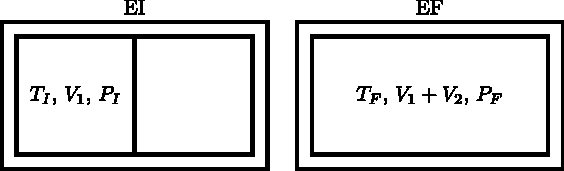
\includegraphics[width=\linewidth]{jgl}
	\end{isd}
	\tcblower
	\psw{%
		Soit $\Sigma = \{\text{gaz + vide}\}$. D'après l'énoncé, $Q = 0$ car
		calorifugé, et $W_p = 0$ car indéformable ($\dd{V} = 0$). Ainsi,
		\begin{gather*}
			\Delta{U} = 0 = \Delta{U}\sup{G.P.}
			\Lra
			C_v \Delta{T}\sup{G.P.} = 0
			\qed
		\end{gather*}
	}%
	\vspace{-15pt}
\end{tcb*}

\begin{tcb}(impl)<lftt>{Cas du système isolé}
	Par définition, un système isolé n'échange pas d'énergie avec l'extérieur. On
	a donc forcément
	\psw{%
		\[
			\boxed{\Delta{U} = 0}
		\]
	}%
	\vspace{-15pt}
\end{tcb}

\subsection{Premier principe entre deux états voisins}

\begin{tcbraster}[raster equal height=rows, raster columns=2]
	\begin{tcb}(defi){États voisins}
		Deux états sont voisins si leurs variables d'état ont des \textbf{valeurs
			très proches}~:
		\[
			\abs{T_f - T_i} \ll T_i
			\qquad
			\abs{P_f-P_i} \ll P_i
			\qquad
			\ldots
		\]
		on parle alors de \textbf{transformation élémentaire}.
	\end{tcb}
	\begin{tcb*}[%
			sidebyside, righthand ratio=.5,
			list entry={\hspace*{-20pt}\protect\rcheck~~Premier principe élémentaire}%
		](prop)'r'{1\ier{} ppe. élémentaire}
		Pour deux états voisins, le premier principe s'exprime avec des variations
		infinitésimales~:
		\psw{%
			\[
				\boxed{\dd{U} = \delta W + \delta Q}
			\]
		}%
		\tcblower
		\begin{center}
			\sswitch{
				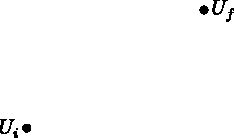
\includegraphics[width=\linewidth]{voisins-plain}
			}{
				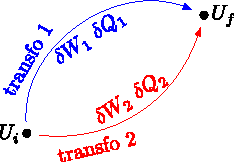
\includegraphics[width=\linewidth]{voisins}
			}
		\end{center}
	\end{tcb*}
\end{tcbraster}

\begin{tcb*}(inte){Notation $\Delta$ ou pas}
	\begin{isd}[sidebyside align=top]
		\tcbsubtitle{\fatbox{\textbf{Grandeur d'état}}}
		Pour une \textbf{grandeur d'état}, on peut parler de sa
		\textbf{variation}, dénotée par un $\Delta$~:
		\[
			\setlength{\fboxsep}{3mm}
			\boxed{\psw{\Delta{U} = U_f - U_i}}
		\]
		Si la variation est \textbf{faible}, on la note par une
		\textbf{différentielle}~:
		\[
			\setlength{\fboxsep}{3mm}
			\boxed{\psw{\dd{U} = C_V \dd{T}}}
		\]
		\tcblower
		\tcbsubtitle{\fatbox{\textbf{Échange d'énergie}}}
		Les \textbf{échanges} n'étant pas \textbf{des grandeurs d'état}\ftn{On ne
			peut pas définir le «~travail d'un état~».}, on n'utilise \textbf{pas} la
		notation
		$\Delta$~:
		\[
			\boxed{\psw{W = -\int P\ind{ext}\dd{V}}}
		\]
		Si le chemin est \textbf{court}, on note l'échange par un $\delta$~:
		\[
			\setlength{\fboxsep}{3mm}
			\boxed{\psw{\delta W = -P\ind{ext}\dd{V}}}
		\]
	\end{isd}
	\begin{center}
		\captionof{table}{Notation de différence selon la grandeur physique}
		\begin{tabular}{ccc}
			\toprule
			\backslashbox{Différence}{Grandeur}
			 &
			\textbf{Grandeur d'état}
			 &
			\textbf{Échanges entre états}
			\\
			\midrule
			Petite
			 &
			$\psw{\dd{U}}$
			 &
			$\psw{\delta W,~\delta Q}$
			\\
			Grande
			 &
			$\psw{\Delta{U}}$
			 &
			$\psw{W,~Q}$
			\\
			\bottomrule
		\end{tabular}
	\end{center}
\end{tcb*}

\begin{tcb*}(appl)<lftt>{Premier principe élémentaire}
	On considère une casserole remplie d’un volume $V = \SI{2}{L}$ d’eau liquide
	posée sur une plaque électrique. On néglige les échanges thermiques avec l’air
	environnant, et on considère que la puissance $\Pc$ des échanges thermiques
	entre le système \{eau + casserole\} et la plaque est constante et vaut
	\SI{500}{W}.
	\smallbreak
	Initialement la température de l’eau est $T_0 = \SI{293}{K}$. On allume la plaque
	à l’instant $t> 0$. On négligera la capacité thermique de la casserole et on
	donne la capacité thermique massique de l’eau liquide $ c =
		\SI{4,18}{kJ.K^{-1}.kg^{-1}}$.
	\begin{enumerate}[label=\sqenumi]
		\item En considérant une transformation élémentaire entre les instants $t$ et
		      $t+\dd{t}$, déterminer l'équation différentielle vérifiée par la température
		      $T$ de l'eau pour $t>0$.
		\item En déduire l'instant $t_1$ pour lequel l'eau commence à bouillir.
	\end{enumerate}
	\tcblower
	\begin{enumerate}[label=\sqenumi]
		\item[m]
			\begin{align*}
				\dd{U} = \psw{\underbracket[1pt]{\cancel{\delta W}}_{=0} + \delta Q}
				\qqeta
				\dd{U} = \psw{mc \dd{T}}
				\\\beforetext{Or}
				\delta Q = \psw{\Pc \dd{t}}
				\qqdca
				\setlength{\fboxsep}{3mm}
				\boxed{\psw{\dv{T}{t} = \frac{\Pc}{\rho Vc}}}
			\end{align*}
			\item[m][20]
			\psw{%
				\[
					T - T_0 = \frac{\Pc}{\rho Vc}t
					\Lra
					\boxed{t_b = (T_b - T_0) \frac{\rho Vc}{\Pc}}
					\Ra
					\xul{t_b = \SI{1340}{s} = \SI{22}{m}}
				\]
			}%
	\end{enumerate}
\end{tcb*}

\section{Transformation monobare et enthalpie d’un système}
Beaucoup de transformations thermodynamiques ont lieu au contact de l’air donc
sous une \textbf{pression extérieure $P\ind{ext}$ constante}. Nous allons voir
une version du premier principe pour ces transformations.
\subsection{Enthalpie et premier principe enthalpique}
\begin{tcb*}(defi){Enthalpie}
	L'enthalpie d'un système d'énergie interne $U$, de pression $P$ et de volume
	$V$ est définie par
	\psw{%
		\[
			\boxed{H = U+PV}
		\]
	}%
	\vspace{-15pt}
	\begin{tasks}[label=\bdmd](3)
		\task \psw{\textbf{énergie}}
		\task \psw{\textbf{grandeur d'état}}
		\task \psw{\textbf{grandeur extensive}}
	\end{tasks}
	On définit donc ses versions molaires et massique~: $H_m = H/n$ et $h = H/m$.
\end{tcb*}

\begin{tcbraster}[raster equal height=rows, raster columns=2]
	\begin{tcb*}[%
			list entry={\hspace*{-20pt}\protect\rcheck~~Premier principe enthalpique}%
		](prop){1\ier{} ppe. enthalpique}
		Pour une transformation \textbf{monobare} pour laquelle il y a
		\textbf{équilibre mécanique dans l'état initial et final} ($P_i = P_f =
		P\ind{ext}$), le premier principe se réécrit~:
		\[
			\psw{\boxed{\Delta{H} = W_u + Q}}
			\qou
			\psw{\boxed{\Delta{H} = Q}}
		\]
	\end{tcb*}
	\begin{tcb*}[%
			list entry={\hspace*{-20pt}\protect\rcheck~~Premier principe enthalpique}%
		](demo)'r'{1\ier{} ppe.\ $H$}
		\psw{%
			\begin{DispWithArrows*}[groups, fleqn, mathindent=-8pt]
				\Delta{U} &= W_p + W_u + Q
				\Arrow{$P\ind{ext} = P_0$}
				\Arrow[jump=3,tikz-code=
						{\draw
							(#1) --++
							(2.5cm,0) |-
							node[pos=.25, sloped] {#3}
							(#2) ;
						}]{On combine}
				\\\beforetext{Or}
				W_p &= -P_0(V_f - V_i)
				\Arrow{$P_i = P_f = P_0$}
				\\\Ra
				W_p & = -P_f V_f + P_iV_i
				\Arrow{$W_p = -\Delta{PV}$}
				\\\Lra
				\Delta{U} &= - \Delta{(PV)} + W_u + Q
				\\\Lra
				\Aboxed{\Delta{H} &= W_u + Q}
				\qed
			\end{DispWithArrows*}
		}%
	\end{tcb*}
\end{tcbraster}

\begin{tcb*}[%
		list entry={\hspace*{-20pt}\protect\rcheck~~Conditions 1\ier{} ppe.\ enthalpique}%
	](impo){Conditions d'application du premier principe enthalpique}
	L’hypothèse d’équilibre mécanique dans l’état initial et final ($P_i = P_f =
		P\ind{ext}$) est \textbf{essentielle} pour que le premier principe prenne
	cette forme~! Par exemple, dans le cas de la seringue compressée brutalement
	par la force $\Ff$, la pression initiale du système n’est pas égale à la
	pression extérieure, qui tiendrait compte de la force $\Ff$~: le premier
	principe enthalpique ne s'applique donc pas.
\end{tcb*}

\subsection{Seconde loi de \textsc{Joule}}

\begin{tcb*}(loi){Seconde loi de \textsc{Joule}}
	Les gaz parfaits et les phases condensées vérifient la seconde loi de
	\textsc{Joule}~: leur \textbf{variation d'enthalpie massique} ou molaire
	ne dépend \textbf{que de la température}.
	\smallbreak
	\begin{isd}[sidebyside align=top, interior hidden](loi)
		\tcbsubtitle{\fatbox{\textbf{Général}}}
		\psw{%
			\[
				\boxed{h = h(T)}
			\]
		}%
		\vspace{-15pt}
		\tcblower
		\tcbsubtitle{\fatbox{\textbf{Gaz parfait}}}
		\psw{%
			\[
				\boxed{H_m = \frac{D+2}{2}RT}
			\]
		}%
		\vspace{-15pt}
	\end{isd}
\end{tcb*}

\begin{tcb*}[sidebyside](prev){Seconde loi de \textsc{Joule}}
	\tcbsubtitle{\fatbox{\textbf{Gaz parfait}}}
	\psw{%
		\begin{gather*}
			\beforetext{}
			U = \frac{D}{2}nRT
			\qet
			PV = nRT
			\\\Lra
			\boxed{H = \frac{D+2}{2}nRT}
			\qed
		\end{gather*}
	}%
	\vspace{-15pt}
	\tcblower
	\tcbsubtitle{\fatbox{\textbf{Phase condensée}}}
	\psw{%
		\begin{gather*}
			\Delta{h} = \Delta{u(T)} + \Delta{(Pv)} = \Delta{u(T)} +
			\underbracket[1pt]{v\Delta{P}}_{\Delta{v} = 0}
			\\
			\beforetext{Or}
			\frac{v\Delta{P}}{\Delta{u}} \ll 1
			\Ra
			\boxed{\Delta{H} \approx \Delta{U}(T)}
			\qed
		\end{gather*}
	}%
	\vspace{-15pt}
\end{tcb*}

\begin{tcb}(exem)<lftt>{Enthalpie de l'eau}
	\begin{align*}
		\beforetext{On a}
		\psw{\frac{\Delta{U}}{m} = c\Delta{T}}
		\qava
		\left\{
		\begin{array}{rcl}
			c         & = & \psw{\SI{4180}{J.K^{-1}.kg^{-1}}}
			\\[.5em]
			\Delta{T} & = & \psw{\SI{100}{K}}
		\end{array}
		\right.
		\Ra
		\xul{
			\Delta{u} = \psw{\SI{4.18e5}{J.kg^{-1}}}
		}
		\\\beforetext{Et}
		\psw{\frac{PV}{m} = \frac{P}{\rho}}
		\qava
		\left\{
		\begin{array}{rcl}
			\Delta{P} & = & \psw{\SI{e5}{Pa}}
			\\[.5em]
			\rho      & = & \psw{\SI{1.0e3}{kg.m^{-3}}}
		\end{array}
		\right.
		\Ra
		\xul{
			v\Delta{P} = \psw{\SI{1e2}{J.kg^{-1}}}
		}
	\end{align*}
	Soit en effet $\Delta{u}\sup{cond} \gg \Delta{(Pv)}\sup{cond}$.
\end{tcb}

\subsection{Capacités thermiques}
% Pour un échantillon de corps pur, l’enthalpie ne dépend que de sa température
% $T$ et de sa quantité de matière $n$. Il est souvent utile de connaître les
% variations de $H$ en fonction de sa température.

\subsubsection{Définition}

\begin{tcb*}[label=defi:cp, sidebyside](defi){Capacité thermique à $P$ constante}
	On appelle \textbf{capacité thermique à pression constante} d'un système fermé la
	grandeur \textbf{extensive}~:
	\psw{%
		\[
			\boxed{C_P = \pdv{H}{T}}
		\]
	}%
	C'est donc la dérivée de l'enthalpie par rapport à la température,
	\textbf{tous les autres paramètres étant constants}.
	\tcblower
	On définit alors également les capacités thermiques \textbf{massique} et
	\textbf{molaire} (intensives) à pression constante~:
	\psw{%
		\[
			c_P = \frac{C_P}{m}
			\qqet
			C_{P,m} = \frac{C_P}{n}
		\]
	}%
\end{tcb*}

\begin{tcb}(inte){Capacité thermique à $P$ constante}
	Physiquement, il s’agit de l’énergie qu’il faut fournir au système (à pression
	et quantité de matière constants) pour augmenter sa température de \SI{1}{K}.
\end{tcb}

\begin{tcb*}(ror){Utilisation des capacités thermiques}
	Comme pour la première loi de \textsc{Joule}, $\Delta{H}$ s'exprime en
	fonction de $C_P$ grâce à la seconde loi de \textsc{Joule}~:
	\vspace{-15pt}
	\psw{%
		\begin{gather*}
			\dd{H} = C_P \dd{T}
			\Lra
			\Delta{H} = \int_{T_i}^{T_f} C_P \dd{T}
			\\\Lra
			\boxed{\Delta{H} = C_P\Delta{T}}
		\end{gather*}
	}%
	\vspace{-15pt}
\end{tcb*}

\subsubsection{Gaz parfait}
\begin{tcb*}(defi){Coefficient adiabatique}
	On appelle \textbf{coefficient adiabatique} ou \textbf{coefficient de
		\textsc{Laplace}} d'un fluide la grandeur
	rapport
	\psw{%
		\[
			\boxed{\gamma = \frac{C_P}{C_V}}
		\]
	}%
\end{tcb*}

\begin{tcbraster}[raster equal height=rows, raster columns=2]
	\begin{tcb*}(prop){Relation de \textsc{Mayer}}
		Les capacités thermiques d'un gaz parfait sont reliées entre elle par la
		relation de \textsc{Mayer}, telle que
		\psw{%
			\[
				\boxed{C_P = C_V + nR}
			\]
		}%
		\vspace{-15pt}
	\end{tcb*}
	\begin{tcb*}[%
			list entry={\hspace*{-20pt}\protect\rcheck~~Relation de \textsc{Mayer}}%
		](demo)'r'{Rela$^\circ$ \textsc{Mayer}}
		\psw{%
			\[
				H = U + nRT
				\Ra
				\dv{H}{T} = \dv{U}{T} + nR
				\qed
			\]
		}%
		\vspace{-15pt}
	\end{tcb*}
\end{tcbraster}

\begin{tcb*}[sidebyside,
		sidebyside align=top](impl){Valeurs de $C_P\sup{G.P.}$ et $\gamma\sup{G.P.}$}
	\tcbsubtitle{\fatbox{\textbf{Monoatomique}}}
	\psw{%
		\begin{gather*}
			C_V = \frac{3}{2}nR
			\quad \Ra \quad
			\boxed{C_P = \frac{5}{2}nR}
			\qet
			\boxed{\gamma = \frac{5}{3}}
		\end{gather*}
	}%
	\tcblower
	\tcbsubtitle{\fatbox{\textbf{Diatomique}}}
	\psw{%
		\begin{gather*}
			C_V = \frac{5}{2}nR
			\quad \Ra \quad
			\boxed{C_P = \frac{7}{2}nR}
			\qet
			\boxed{\gamma = \frac{7}{5}}
		\end{gather*}
	}%
\end{tcb*}

\begin{tcbraster}[raster equal height=rows, raster columns=2]
	\begin{tcb*}[%
		list entry={\hspace*{-20pt}\protect\rcheck~~{Expressions de $C_V\sup{G.P.}$
		et $C_P\sup{G.P.}$}}%
		](ror){$C_V\sup{G.P.}$ et $C_P\sup{G.P.}$}
		Les capacités thermiques d'un gaz parfait s'expriment en fonction de $\gamma$,
		tel que
		\[
			\psw{\boxed{C_V = \frac{nR}{\gamma-1}}}
			\qqet
			\psw{\boxed{C_P = \frac{\gamma nR}{\gamma-1}}}
		\]
	\end{tcb*}
	\begin{tcb*}[%
		list entry={\hspace*{-20pt}\protect\rcheck~~{Expressions de $C_V\sup{G.P.}$
		et $C_P\sup{G.P.}$}}%
		](demo)'r'{$C_V\sup{G.P.}$ et $C_P\sup{G.P.}$}
		\psw{%
			\begin{gather*}
				C_P = C_V + nR
				\qet
				C_P = \gamma C_V
				\\\Lra
				C_V (\gamma-1) = nR
				\\\Lra
				\left\{
				\begin{array}{rcl}
					C_V & = \DS \frac{nR}{\gamma-1}
					\\
					C_P & = \DS \frac{\gamma nR}{\gamma-1}
				\end{array}
				\right.
			\end{gather*}
		}%
	\end{tcb*}
\end{tcbraster}

\subsubsection{Phases condensées}
\begin{tcb*}[%
		list entry={\hspace*{-20pt}\protect\rcheck~~Capacités thermiques phase cond.}%
	](prop){Capacités thermiques phase condensée}
	On a démontré que l'enthalpie d'une phase condensée était similaire à son
	énergie interne, on a donc automatiquement
	\psw{%
		\[
			\boxed{C_P \approx C_V = C = \cte}
		\]
	}%
\end{tcb*}

\begin{tcb*}(defi){Calorimètre}
	\noindent
	\begin{minipage}[c]{.68\linewidth}
		Un calorimètre est un récipient composé en général d’une paroi extérieure et
		d’une cuve intérieure, fermé par un couvercle percé de petites ouvertures
		permettant d’introduire des appareils mécaniques.
		\begin{itemize}
			\item Sur une courte durée, on peut \textbf{négliger les échanges
				      termiques} avec l'extérieur~;
			\item Des ouvertures assurent une \textbf{transformation monobare}~;
			\item On exprime la capacité du calorimètre par sa \textbf{valeur en
				      eau} $m_0$~:
			      \[
				      C\ind{calo} = m_0 c\ind{eau,liq}
			      \]
		\end{itemize}
	\end{minipage}
	\hfill
	\noindent
	\begin{minipage}[c]{.30\linewidth}
		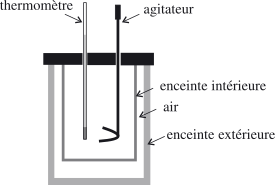
\includegraphics[width=\linewidth]{calo_def}
	\end{minipage}
\end{tcb*}

\begin{tcb*}(appl)<lftt>{Calorimétrie}
	Dans un calorimètre parfaitement isolé de masse en eau $m_0 = \SI{24}{g}$, on
	place $m_1 = \SI{150}{g}$ d'eau à $T_1 = \SI{298}{K}$. On ajoute $m_2 =
		\SI{100}{g}$ de cuivre à $T_2 = \SI{353}{K}$, avec $c_{\ce{Cu}} =
		\SI{385}{J.K^{-1}.kg^{-1}}$. On cherche la température d'équilibre $T_f$.
	\begin{enumerate}[label=\sqenumi]
		\item Exprimer $\Delta{H}\ind{eau}$ en fonction de $m_1$, $c\ind{eau}$,
		      $T_1$ et $T_f$.
		\item Exprimer $\Delta{H}_{\ce{Cu}}$ en fonction de $m_2$, $c_{\ce{Cu}}$,
		      $T_2$ et $T_f$.
		\item Exprimer $\Delta{H}\ind{calo}$ en fonction de $m_0$, $c\ind{eau}$,
		      $T_1$ et $T_f$.
		\item Justifier que $\Delta{H}\ind{tot} = 0$.
		\item En déduire $T_f$.
	\end{enumerate}
	\tcblower
	\begin{enumerate}[label=\sqenumi]
		\item[m]
			\psw{%
				\begin{gather*}
					\boxed{\Delta{H}\ind{eau} = m_1c\ind{eau} (T_f - T_1)}
				\end{gather*}
			}%
			\vspace{-25pt}
		\item[m]
			\psw{%
				\begin{gather*}
					\boxed{\Delta{H}_{\ce{Cu}} = m_2c_{\ce{Cu}} (T_f - T_2)}
				\end{gather*}
			}%
			\vspace{-25pt}
		\item[m]
			\psw{%
				\begin{gather*}
					\boxed{\Delta{H}\ind{calo} = m_0c\ind{eau} (T_f - T_1)}
				\end{gather*}
			}%
			\vspace{-25pt}
		\item \psw{%
			      Calorimètre isolé donc $Q = 0$, et pas de variation de volume donc
			      $W_p = 0$ et pas d'autres travaux donc $W_u = 0$~:
			      \[
				      \boxed{\Delta{H}\ind{tot} = 0}
			      \]
		      }%
		\item[m]
			\psw{%
				\begin{align*}
					(m_1 + m_0)c\ind{eau} (T_f - T_1) + m_2c_{\ce{Cu}}(T_f - T_2)
					    & = 0
					\\\Lra
					T_f \left( (m_1+m_0)c\ind{eau} + m_2c_{\ce{Cu}} \right)
					    & =
					T_1 \left( m_1+m_0 \right)c\ind{eau} + T_2m_2c_{\ce{Cu}}
					\\\Lra
					\Aboxed{
					T_f & =
					\frac{\left( m_1+m_0 \right)c\ind{eau}T_1 + m_2c_{\ce{Cu}}T_2}
					{(m_1+m_0)c\ind{eau} + m_2c_{\ce{Cu}}}
					}
					\\
					\makebox[0pt][l]{$\phantom{\AN}\xul{\phantom{T_f = \SI{301}{K}}}$}
					\AN
					T_f & = \SI{301}{K}
				\end{align*}
			}%
	\end{enumerate}
	\vspace{-25pt}
\end{tcb*}

\end{document}
